\documentclass[12pt]{article}

\usepackage{listings}
\usepackage{color}
\usepackage{graphicx}
\usepackage[margin=0.7in]{geometry}
\usepackage[english]{babel}
%\usepackage[utf8x]{inputenc}
\usepackage{amsmath}
\usepackage{graphicx}
\usepackage[colorinlistoftodos]{todonotes}
\usepackage{listings}


\begin{document}
\begin{titlepage}

\newcommand{\HRule}{\rule{\linewidth}{0.6mm}} % Defines a new command for the horizontal line, Thickness can be changed

\center % Center everything on the page
 
%----------------------------------------------------------------------------------------
%	HEADING
%----------------------------------------------------------------------------------------
\textsc{\LARGE ELP 780}\\[0.5cm] % Course Code

\textsc{\huge Software Lab}\\[1.5cm] % software lab course name



%----------------------------------------------------------------------------------------
%	LOGO
%----------------------------------------------------------------------------------------


\includegraphics[scale=.5]{logo.png}\\[1cm] % IIT Delhi Logo
\LARGE{INDIAN INSTITUTE OF TECHNOLOGY}\\
{\Large{NEW DELHI}}\\


%----------------------------------------------------------------------------------------
%	Assignment Number
%----------------------------------------------------------------------------------------

\HRule \\[0.4cm]
{ \large \textbf {Assignment 8}}\\[0.4cm] % Title of your document
\HRule \\[1cm]
%----------------------------------------------------------------------------------------
%	DATE SECTION
%----------------------------------------------------------------------------------------

{\large \today}\\[3cm] % Date
 
%----------------------------------------------------------------------------------------
%	Personal Details
%----------------------------------------------------------------------------------------

\begin{minipage}{0.4\textwidth}
\begin{flushleft} \Large
\emph{Name:}
\textbf{Priya Kumari}%My Name
\end{flushleft}
\end{minipage}
~
\begin{minipage}{0.4\textwidth}
\begin{flushright} \Large
\emph{Entry Number:} \\
\textbf{2017EET2305} % Entry Number
\end{flushright}
\end{minipage}\\[2cm]

\HRule



%----------------------------------------------------------------------------------------
\vfill % Fill the rest of the page with whitespace

\end{titlepage}
  
\pagebreak
\tableofcontents
\pagebreak

\pagenumbering{arabic}
\section{Problem Statement 1}
{
\textbf{}
Question 1:
IIT Delhi, has just got the strongest computer. The professors in charge wants to check the computational capacity of the computer. So, they decided to create the problem which is to be given as an assignment to students. Can you help the professor to check the computation capability of the computer?
\\
A valid cross is defined here as the two regions (horizontal and vertical) of equal lengths crossing over each other. These lengths must be odd, and the middle cell of its horizontal region must cross the middle cell of its vertical region.
\\
Find the two largest valid crosses that can be drawn on smart cells in the grid, and return two integers denoting the dimension of the each of the two largest valid crosses. In the above diagrams, our largest crosses have dimension of 1,  5 and 9 respectively .
\\
}
\subsection{Assumptions}
{
The two crosses cannot overlap, and the dimensions of each of the valid crosses should be maximal.


}

\subsection{Program Structure}
{
\begin{enumerate}
\item take the values of k1 l2 k3
\item take the string
\item divide string into group1 group2 group3
\item rotate the 3 strings
\item replace to make result
   

 
\end{enumerate} 
}

\newpage
\subsection{Flowchart}
\begin{figure}[h]
	\centering
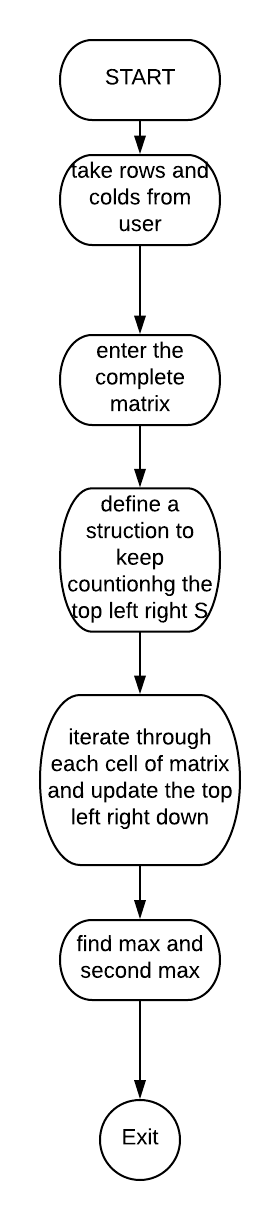
\includegraphics[width=0.3\textwidth]{ps1flow.png}\\
\end{figure}
\newpage

\subsection{Constraints}
{

2 <= n <= 105\\
2 <= m <= 105
}
\subsection{Input}
{

\textbf{Input format} \\
The first line contains two space-separated integers,  n and m. 
Each of the next  lines n contains a string of  m characters where each character is either S (Smart) or D (Dull). These strings represent the rows of the grid. If the jth character in the ith  line is S, then  (i,j) is a  cell smart. Otherwise it's a  dull cell.
}
\subsection{Output}
{
\textbf{Input format} \\
Find two valid crosses that can be drawn on smart cell of the grid, and return the dimension of both the crosses in the reverse sorted order(i.e. First Dimension should be the larger one and other should be smaller one).\\
}
\subsection{Input Screenshot}
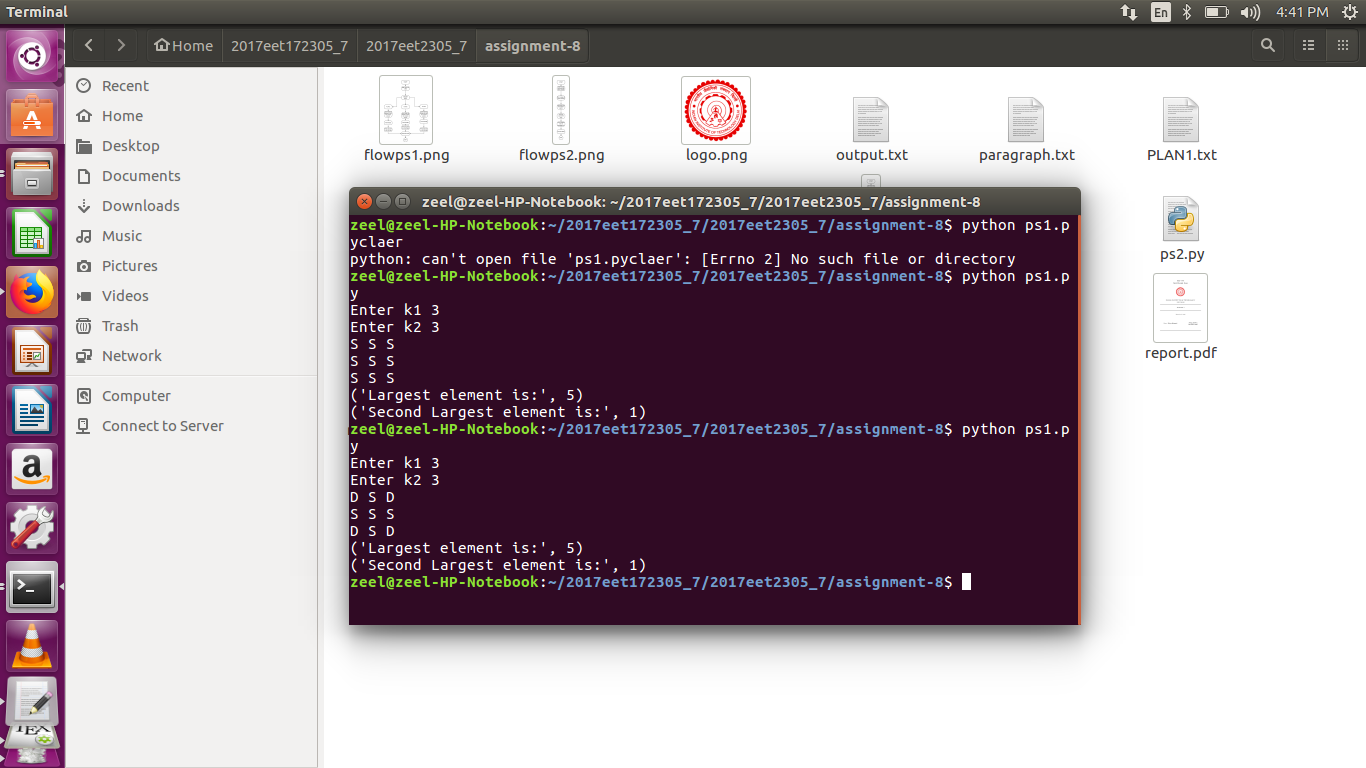
\includegraphics[width=0.5\textwidth]{ps1screenshot.png}

\subsection{Output Screenshots}
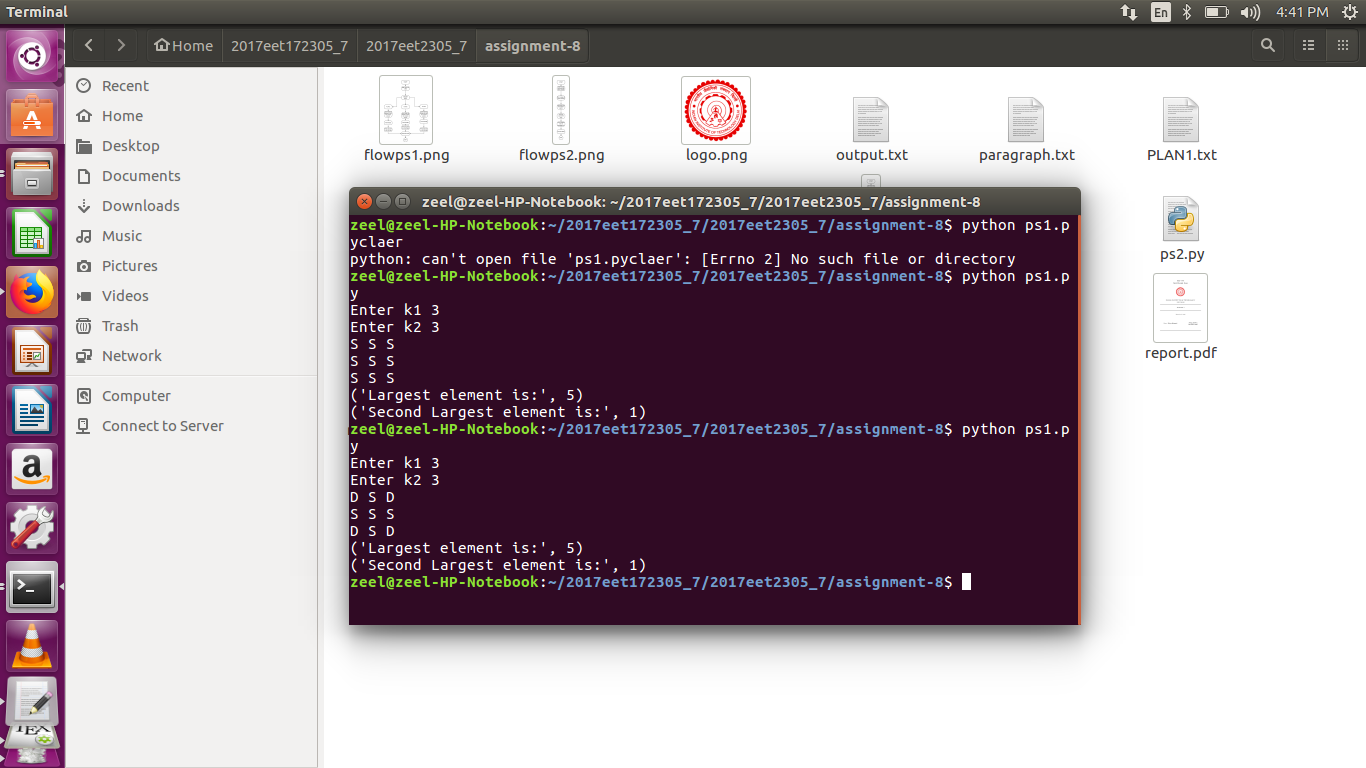
\includegraphics[width=0.5\textwidth]{ps1screenshot.png}
{
\begin{center}
    
\end{center}    
}



\pagebreak
\section{Problem Statement 2}
{\textbf{}Question 2:
After, getting mix results of valid crosses, professors decided to test the computation abilities on one more problem. This time professors wanted to test the decryption capabilities of the computer.\\
Encryption of  a message requires three keys, k1, k2, and k3. The 26 letters of English and underscore are divided in three groups,  [a-i] form one group, [j-r] a second group, and everything else ([s-z] and underscore) the third group. Within each group the letters are rotated left by ki positions in the message. Each group is rotated independently of the other two. Decrypting the message means doing a right rotation by ki positions within each group.

}



\subsection{Assumptions}
{
 Rotating letters in one group will not change any letters in any of the other groups.


}

\subsection{Program Structure}
{
\begin{enumerate}
\item enter rows and cols from user
\item enter the S D matrix
\item define a structure with left right up down values
\item iterate through each cell and update the left right top down
\item store the values in a list
\item find max and second max

\end{enumerate} 

}
\newpage
\subsection{Flowchart}
\begin{figure}[h]
	\centering
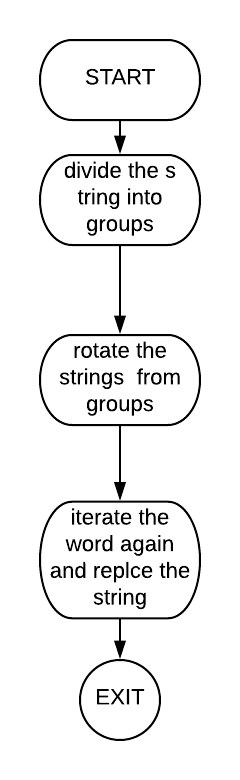
\includegraphics[width=0.2\textwidth]{ps2flow.png}\\
\end{figure}
\newpage


\subsection{Output Format}
{
\textbf{} \\
1 <= Length of the string <=150\\
1<= ki <=150 (i=1,2,3)
}
\subsection{Input Format}

{
\textbf{} \\
All input strings comprises of only lowercase English alphabets and underscores


}


\subsection{Output Format}
{
\textbf{} \\
For each encrypted message, the output is a single line containing the decrypted string.
}

\subsection{Input Screenshot}
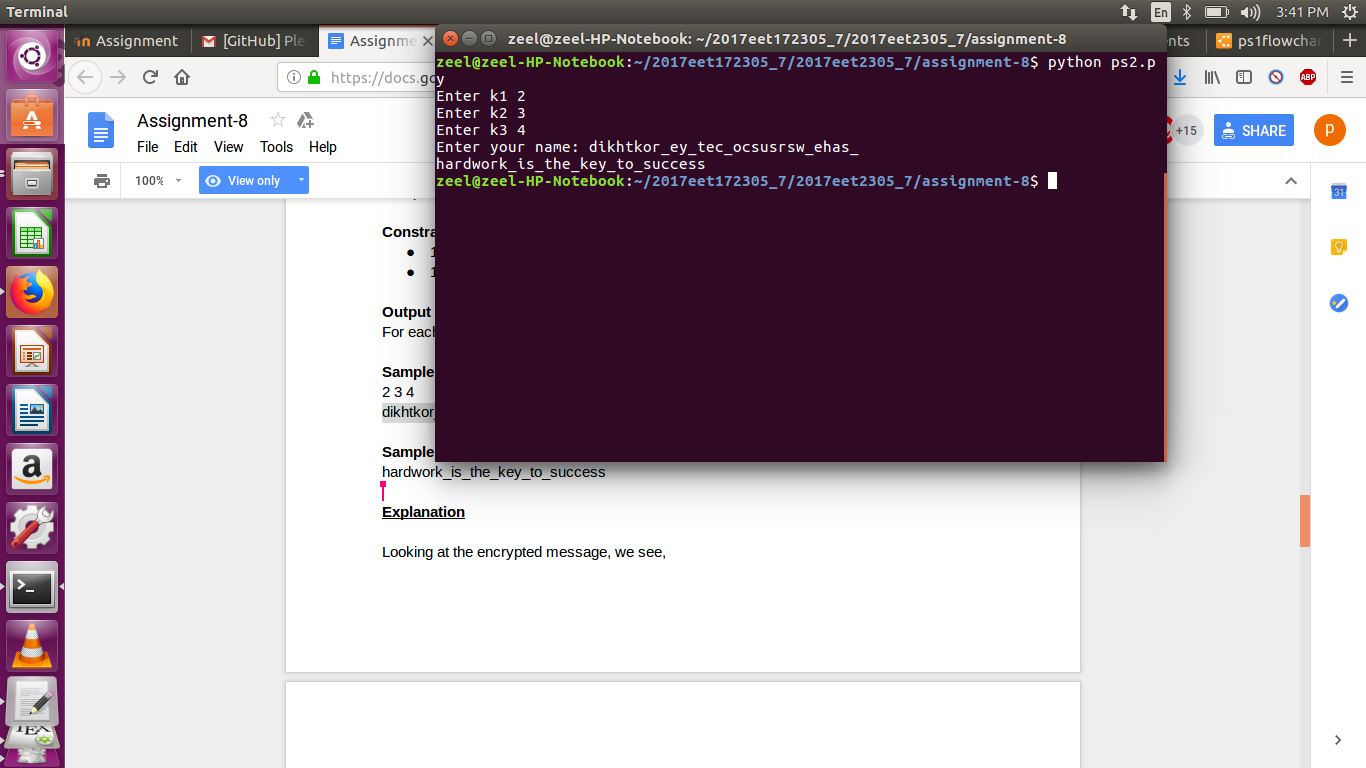
\includegraphics[width=0.5\textwidth]{ps2screenshot.png}

\subsection{Output Screenshot}
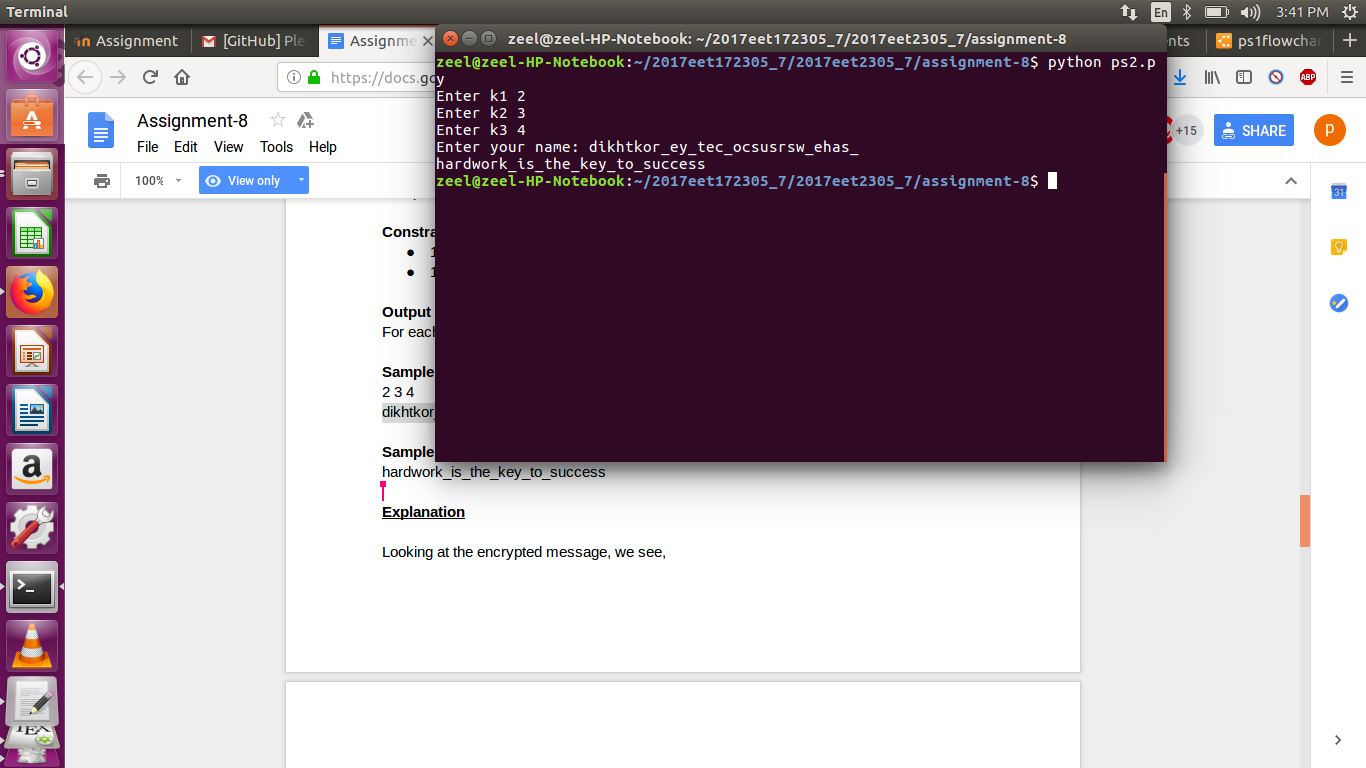
\includegraphics[width=0.5\textwidth]{ps2screenshot.png}
{
\begin{center}
    
\end{center}    
}

\newpage
\section{Code}
\textbf{code1}
\lstinputlisting[language=c]{ps1.py}  
\textbf{code2}
\lstinputlisting[language=c]{ps2.py}  

\newpage
\section{Bibliography}
{
\begin{enumerate}
\item https://www.stackoverflow.com
\item https://code2flow.com
\item https://www.geeksforgeeks.org/python-maximum-minimum-elements-position-list/
\item https://stackoverflow.com/questions/33181350/quickest-way-to-find-the-nth-largest-value-in-a-numpy-matrix
\end{enumerate}
}
\end{document}